%
% File coling2020.tex
%
% Contact: feiliu@cs.ucf.edu & liang.huang.sh@gmail.com
%% Based on the style files for COLING-2018, which were, in turn,
%% Based on the style files for COLING-2016, which were, in turn,
%% Based on the style files for COLING-2014, which were, in turn,
%% Based on the style files for ACL-2014, which were, in turn,
%% Based on the style files for ACL-2013, which were, in turn,
%% Based on the style files for ACL-2012, which were, in turn,
%% based on the style files for ACL-2011, which were, in turn, 
%% based on the style files for ACL-2010, which were, in turn, 
%% based on the style files for ACL-IJCNLP-2009, which were, in turn,
%% based on the style files for EACL-2009 and IJCNLP-2008...

%% Based on the style files for EACL 2006 by 
%%e.agirre@ehu.es or Sergi.Balari@uab.es
%% and that of ACL 08 by Joakim Nivre and Noah Smith

\documentclass[11pt]{article}
\usepackage{coling2020}
\usepackage{times}
\usepackage{amsmath,amsfonts,amssymb}
\usepackage{url}
\usepackage{latexsym}
\usepackage{hyperref}
\usepackage[noabbrev,capitalize]{cleveref}
\usepackage{graphicx}
\usepackage{natbib}
\usepackage{subcaption}
\usepackage{pgfplots}

\newcommand\jp[1]{(\textbf{JP:} #1)}
%\setlength\titlebox{5cm}
%\colingfinalcopy % Uncomment this line for the final submission

% You can expand the titlebox if you need extra space
% to show all the authors. Please do not make the titlebox
% smaller than 5cm (the original size); we will check this
% in the camera-ready version and ask you to change it back.


\title{Composing Byte-Pair Encodings for Morphological Sequence Classification}


\author{Adam Ek \and Jean-Philippe Bernardy\\
	Centre for Linguistic Theory and Studies in Probability,\\
	Department of Philosophy, Linguistics and Theory of Science,\\
	University of Gothenburg,\\
	\texttt{\{adam.ek, jean-philippe.bernardy\}@gu.se}}

\date{}

\begin{document}
	\maketitle
	
	\begin{abstract}
		This document contains the instructions for preparing a paper submitted
		to COLING-2020 or accepted for publication in its proceedings. The document itself
		conforms to its own specifications, and is therefore an example of
		what your manuscript should look like. These instructions should be
		used for both papers submitted for review and for final versions of
		accepted papers. Authors are asked to conform to all the directions
		reported in this document.
	\end{abstract}
	
	\section{Introduction}
	\label{intro}
	
	\textbf{Things added to model:}
	\begin{itemize}
		\item Adaptive learning rate
		\item Dropouts
		\item Trained character representations (?)
	\end{itemize}
	
	\textbf{Things to add:}
	\begin{itemize}
		\item (results) With fine-tuning/without fine-tuning
		\item (data) Data statistics: number of MSD-tags 
		\item (data) Pick other datasets, try to match dataset sizes better (100k-150k train examples, turkish very small atm)
	\end{itemize}

            Since its introduction [CITE:TODO], the transformer model
     \citep{vaswani2017attention} has emerged as the dominant
     architecture for statistical language model, gradually displacing
     recurrent neural networks, in particular the LSTM and its
     variants. The transformer owes its success to several factors,
     including the availability of pretrained models, which
     effectively yield rich contextual word embeddings. Such
     embeddings can be used as is (for so-called feature extraction),
     or the pre-trained models can be fine-tuned to specific
     applications.

    	At the same time as transformer models became popular, the
     tokenization of natural language texts have shifted away from
     methods explicitly oriented on words or morphemes. Rather,
     statistical approaches are favoured to splits strings of
     characters into units which are not necessarily meaningful
     linguistically, but rather have statistically balanced
     frequencies. For example, the word "scientifically" may be
     composed of the tokens: "scient", "ifical", "ly" --- here the
     central token does not correspond to a morpheme.
        %
            Rather than identifying complete words or morphemes, it
     aims to find sub-word units occurring significantly
     often. Typical approaches to composing tokens from sub-token
     units have focused on combining character n-grams
     \citep{bojanowski2017enriching}, while other approaches have
     looked at splitting words into \textit{roots} and
     \textit{morphemes}, and then combining them. In this paper, we
     consider in particular Byte-Pair Encodings (BPE)
     \citep{sennrich2015neural}, which take another approach. One does
     not specifically look for either character n-grams or morphs, but
     rather it aim to split a corpus $\mathcal{C}$ into $N$ tokens,
     where $N$ is user defined. [EXPAND]

            One issue with statistical tokenization is that one is
     seldom interested in the encoding, but rather in the semantically
     meaningful units in the original texts. Thus the question of
     mapping data about the token back to the original text arises.
        
    	In this paper we explore how to combine Byte-Pair Encodings
     from a transformer model to perform sequence classification,
     which is used in particular in the popular BERT model
     \citep{devlin2018bert}. For our purposes, the goal in sequence
     classification is to assign a label to every word in a
     sentence. When we are using byte-pair encoding (or similar
     sub-token representations) we must then find some way of
     combining the units that build the word, before it is eventually
     assigned a label. Coming back to our example, we must map the
     feature-set assigned (depending on the context) to "scient",
     "ifical", "ly". Then this combined feature set is mapped to a
     class for the whole word ``scientifically''.

    	To our knownledge, this is a little-studied
     problem. [citet:TODO] have only brushed the surface by reporting
     that few differences are found between different methods. In this
     paper we wish to explore the problem in further detail and
     identify what effect different methods have on the final
     performance of a model.

    %In this paper we explore the transformer model applied to sequence classification. In sequence classification a dataset is split into words (or tokens) and each word is assigned a label. 
    %Neural model can predict the label of a word by assigning it a representation and passing it through the network. However, the transformer model use byte-pair encoding (BPE) \cite{sennrich2015neural}, or some variation of it \citep{devlin2018bert}, to tokenize text. 
    %BPE tokens are sub-strings that occur significantly often in the corpus, and does not correspond directly to words. 
    %
    %In sequence classification, we need to assign a label to the word "scientifically". But the word is now composed of three BPE embeddings, so to predict a label for the word we need to compose all of the BPE embeddings into one representation.
    
    %In this project is to explore six different methods of creating word representations from multiple BPE embeddings.
	
%%%
    %Typically, the transformer model use some variation of byte-pair endings (BPE)  to split sentences into tokens. For non-bpe tokenization schemas typically words are selected based on white-space. This is convenient in sequence classification or parsing where for each word some label is assigned. 
    %In the BPE schema on the other hand a word (which has a label attached to it in some dataset) may be split into two or more BPE-tokens. 
    %The BPE vocabulary is usually selected such that significantly common sub-strings are saved. To create words using a BPE vocabulary, sub-strings are combined with each other.
    
    %In this project we explore how to compose embeddings of BPE tokens into word representations. More specifically, in cases when a word is associated with several BPE embeddings (for example: the word "scientifically" may be composed of the the BPE tokens: ["scient", "ifical", "ly"]) how do we combine the BPE embeddings to create a word representation ("scientifically") which we assign a label to.
    
    %\paragraph{Task:} We explore combination of BPE embeddings with the task of Morphological-Tagging-in-Context \citep{mccarthy2019sigmorphon}. 
    %The task is simply to predict the morphological features (such as case, number person, ...) of each word (as defined in the dataset) given the sentence which the word occur in.
    
        \paragraph{Task:} In this paper we further focus on the task
        of morphological sequence classification. Morphological
        tagging involves identifying a set of morphological features
        that a word possesses, such as number, person, case, etc. In
        many languages, morphological features primarily depend on the
        affixes of words. However, conversely, the morphological class
        is not determined by the word affixes, nor the whole word. In
        many cases, the context of the sentence will affect which
        class should be assigned to a word.

        \paragraph{Data:} For the task we will use the Universal
        Dependencies dataset \citep{nivre2018} annotated with the
        UniMorph schema \citep{mccarthy2018marrying}. We are
        interested both in the general effects of using different
        composition methods, and whether some methods favor languages
        with certain typologies. To explore this, we take a sample of
        eight languages from the Universal Dependencies dataset. Four
        of them use a \textit{fusional} morphology, meaning that an
        affix may be indicative of one or more morphological
        features. Four of them use an \textit{agglutinative}
        morphology, meaning that each affix is mapped to one and only
        one morphological feature.
    
   	The fusional languages that we consider are Arabic, Czech,
        Polish and Spanish, and the agglutinative languages that we
        consider are Finnish, Basque, Turkish and Estonian. The size
        of the dataset \jp{in original words?}  and the average number
        of BPE tokens per word are shown in \cref{tab:data}.
    
    	\begin{table} % JP it's better to leave placement to the tex engine and the style sheet. (unless there is a real problem doing so)
		\centering
		\begin{tabular}{l|lrrrrr}
			Language & Typology & $\frac{BPE}{word}$ & Tags & Train & Validation & Test \\
			\hline
			Finnish-TDT     & Agglutinative & 1.98 & 591 & 161791 & 19876 & 20541 \\
			Basque-BDT      & Agglutinative & 1.79 & 919 & 97336 & 12206 & 11901 \\
			Turkish-IMST    & Agglutinative & 1.73 & 1056 & 46417 & 5708 & 5734 \\
			Estonian-EDT    & Agglutinative & 1.86 & 512 & 346986 & 43434 & 43825 \\
            Arabic-PADT     & Fusional & 1.39 & 300 & 225494 & 28089 & 28801  \\
			Czech-CAC       & Fusional & 1.77 & 990 & 395043 & 50087 & 49253 \\
			Polish-LFG      & Fusional & 1.75 & 634 & 104730 & 13161 & 13076 \\
			Spanish-AnCora  & Fusional & 1.25 & 177 & 439925 & 55196 & 54449 \\
        \end{tabular}
		\caption{\label{tab:data} Treebank statistics showing the language typology, average number of BPE tokens per word, the number of morphological tags and the size of the datasets.}
	\end{table}
    
        The fusional languages where chosen such that two of them
        (Czech and Polish) have a higher BPE per token ratio than the
        other two (Arabic and Spanish). We make this choice because
        one factor that impacts the accuracy obtained by a composition
        method may be the BPE per token ratio.  By having both
        fusional and agglutinative languages with similar BPE per
        token ratio we can take this variable into account properly in
        our analysis.

	\section{Method}
	\label{method}
        \jp{This section should be revised, it's quite unclear what
          the model is. It would help to: 1. describe the model in
          computational order 2. use $f$ consistently to denote the
          part which can vary in the model.}
        
	In this section we present the model used for sequence
        classification, the methods that we use to compose BPE
        embeddings, and how we trained the model.
	
	\paragraph{Transformer model}
        	For the task we use the XLMR
     \citep{conneau2019unsupervised} model\footnote{We use the
     huggingface implementation [CITE/LINK]}. XLMR is a masked
     language model based on the transformer (specifically, RoBERTa
     \citep{liu2019roberta}), and trained on data from 100 different
     languages, using a shared vocabulary. All languages we test are
     included in XLMR model. In this experiment we use
     \textsc{XLMR}$_{base}$ model. It has 12 encoder layers, 16 (?)
      attention heads and use 768 dimensions for its hidden size.
	
	\subsection{Model}
	For morphological tagging we use the XLMR base model with a
        classification module on top. The classification module is an
        LSTM followed by a two layer linear transformation.\jp{Is the
          LSTM always there? I thought mean and sum were used as
          well?}
	
	The model that we use to predict morphological features is as
        follows. For each sentence we extract $n$ BPE embeddings $x^0$
        to $x^{n-1}$. from $XLMR_{base}$, and then align them to
        words.  We then feed all words which consist of more than one
        BPE embedding to a function $f$ which combines the BPE
        embeddings. This produces one embedding per word, which we
        concatenate with character features generated by a character
        LSTM. We then pass the BPE features concatenated with the
        character features to an LSTM to extract contextual
        features.\jp{Again, is this active always?}  We pass the LSTM
        outputs to a linear transformation layer that computes scores
        for each class in the output. We then use a softmax layer to
        assign probabilities, and compute the loss accordingly.
	
	An outline of the model is presented in \cref{fig:model}, in
        the outline $f$ represents the different methods we use to
        combine BPE embeddings.
	
	\begin{figure}[h!]
		\centering
		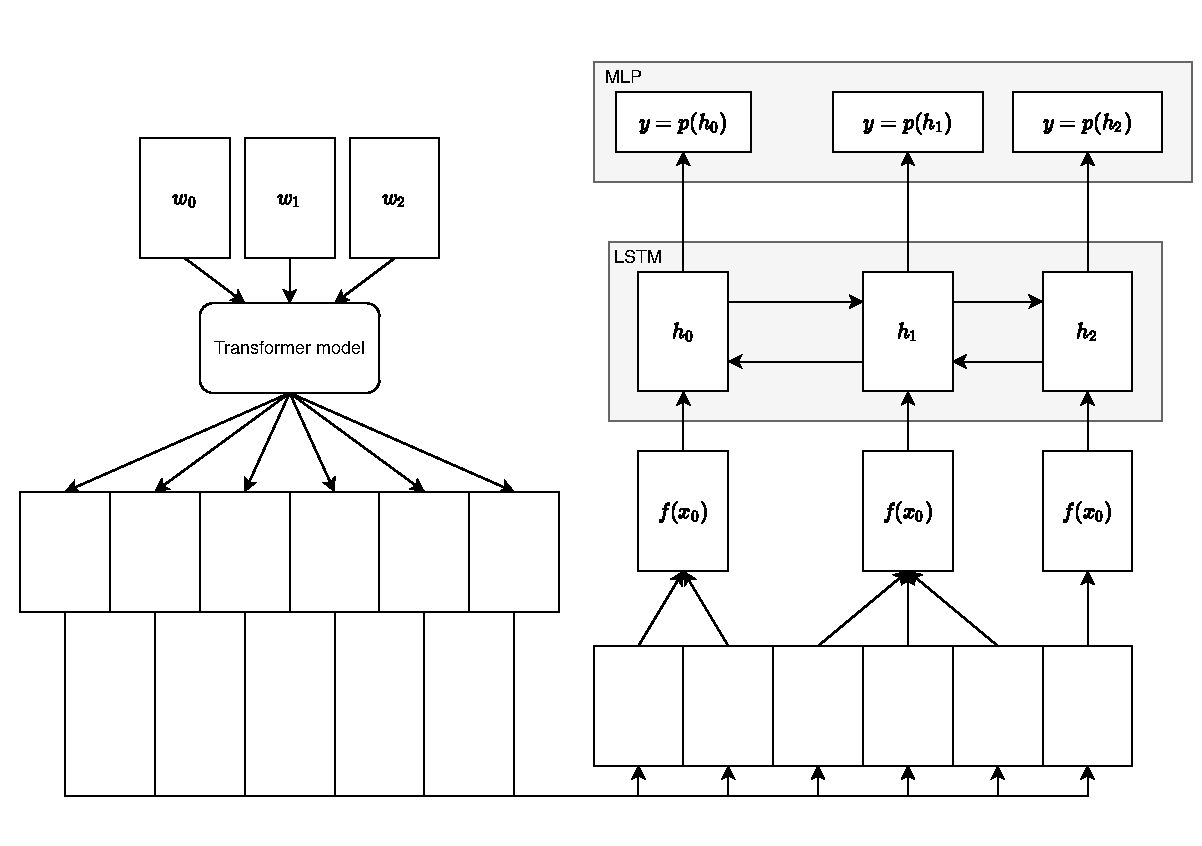
\includegraphics[scale=0.5]{model-outline.pdf}
		\caption{\label{fig:model} Procedure outline}
	\end{figure}
	
	\subsubsection{BPE features}

            As mentioned previously, we look at methods for composing
     embeddings of BPE tokens into word embeddings. The XLMR model use
     12 layers to compute an embedding for a BPE token, and it has
     been shown in previous research \citep{kondratyukstraka,
     raganato2018analysis} [Find 1 or 2 more citations] that the
     different layers of the transformer model encode different types
     of information. To take advantage of this we compute BPE
     embeddings as a weighted sum of layer representations.  That is,
     we initialize a parameter from a standard normal distribution $w$
     (AE NOTE: also tried with a parameter of only 1's, but random was
     better) of size $l$, where $l$ is the number of laters in the
     transformer model. Where $r_{ji}$ is the layer representation at
     layer $j$ and token position $i$, we calculate the weighted sum
     as follows:

    \begin{equation}
		x_i = \sum_{1}^{J} softmax(w)_j r_{ji}
	\end{equation}

        Where $softmax(w)_j$ indicate the softmax of the learned
     importance of layer $j$. After we have computed a weighted sum for
     each BPE token we proceed to combine them into the tokens as they
     appear in the data. To align BPE tokens to tokens in the text we
     use a simple alignment algorithm [It's super simple...].
    
%	When extracting features from XLMR we compute a weighted sum
%        of the layer representations. This is inspired by previous
%        work showing that the different layers in language models
%        encode different kinds of information \jp{citation
%          needed}. That is, we use a parameter $w$ of dimension $l$
%        \jp{where l is the number of layers in the transformer
%          model?}, such that $w_i$ indicates the importance of the
%        layer $i$. We calculate the weighted sum for each bpe
%        representation layerwise:
	
%	\begin{equation}
%		x_i = \sum_{1}^{J} softmax(c)_j l_{ji}
%	\end{equation}
%	\jp{How is $w$ initialised? How is it optimised? End-to-end
%          training? Add a forward reference to the training section and explain it there.}


        We look at three method in particular, summation and averaging
     along a dimension, and using an RNN. Summation and mean have been
     used in previous work, but using an RNN have not been explored
     before to our knowledge.
    
    	\paragraph{Sum:} For the sum method, we use an element-wise
     sum. That is, we take the sum for each dimension of the BPE
     embeddings separately. Thus, for token $i$ we calculate a
     composite embedding by summing over dimensions $0,\ldots,N$:
	
	\begin{equation}
	f(x)_i = \sum_{j=1}^{n} x_i^j
	\end{equation}
	

    	\paragraph{Mean:} In the mean method we calculate the sum and
     divide by the number of BPE embeddings in the word. Thus, for
     token $i$ we calculate a composite embedding by averaging over
     dimensions $0,\ldots,N$:
	
	\begin{equation}
	f(x)_{i} = \frac{1}{n}\sum_{j=1}^{n} x_i^j
	\end{equation}
	
	
	\paragraph{RNN:} For this method we employ a bidirectional LSTM
        to compose the BPE embeddings. For each multi-BPE
        token, we pass the sequence of BPE embeddings through an LSTM
        and use the final output as the word representation. 
    
	\subsubsection{Character features}
    	In addition to layer attention we use a character LSTM to
     extract a word representation based on characters. The final
     representation that we pass to the word-LSTM is the concatenation
     of the word representation based on BPE compositions and
     characters,
     $w_i = \text{concat}(f(bpe_0,...,bpe_K), f(c_0, ..., c_M))$
	
	\subsubsection{Label smoothing}
    	Given that many of the languages have a large number of
     morphological tags, we want to prevent the model from growing
     overconfident for certain classes. To address this issue we
     introduce label smoothing \citep{szegedy2016rethinking}, that is,
     instead of the incorrect classes having 0 probability and the
     correct class $100\%$ probability we let each of the incorrect
     classes have a small probability.

        %The correct class is then assigned the probability $t$ by
     %$(1-\alpha)t + \alpha / |C|$ where $|C|$ is the number of
     %classes. \jp{I don't understand this formula (and I botched the
     %sentence trying to fix it :/ ... What is $t$? I was expecting
     %that you'd give the formula for the probability of the correct
     %class, but apparently I am mistaken.)}

                Let $\alpha$ be our smoothing value, then given a
     one-hot encoded target vector $t$ of size $(N,C)$ where $N$ is
     the number of examples and $C$ the number of classes we calculate
     the smoothed probabilities as:

    \begin{equation}
        t_{smooth} = \frac{(1-\alpha)t + \alpha}{C}
    \end{equation}

            The intuition is that we remove $1-\alpha$ from the
     correct class then distribute $\alpha$ uniformly among all
     classes. 

	\subsection{Training}
	
        	When fine-tuning the model we freeze the XLMR parameters
     for the first epoch.  When training the model we use cosine
     annealing learning rate with restarts every epoch, that is, the
     learning rate starts high then incrementally decrease to $1e-12$
     during N steps, where N is the number of batches in an epoch. We
     use a learning rate of $0.001$ for the word LSTM, classification
     layer and BPE combination module (when an RNN is used), for the
     transformer we use a lower learning rate of $1e-06$.

    %a_parser.add_argument('--xlmr_dropout', type=float, default=0.2) # number of input tokens changed to <unk>
    %a_parser.add_argument('--layer_dropout', type=float, default=0.1) # p that layer j is set to 0.
    %a_parser.add_argument('--layer_repr_dropout', type=float, default=0.4) # dropout for w (in all layers)
    %a_parser.add_argument('--transform_dropout', type=float, default=0.5) # dropout before predict(w)
    %a_parser.add_argument('--char_dropout', type=float, default=0.4) # dropout on w after char rnn
    %a_parser.add_argument('--bpe_dropout', type=float, default=0.4) # dropout on w after bpe composition
    
	\begin{table}[h]
		\centering
		\begin{tabular}{lr}
			Parameter & Value \\
			\hline
			Epochs & 15 \\
			Batch size & 4 / 32 \\
			Character representation size & 128 \\
            Word LSTM size & 1536 \\
            Linear transform size & 1536 \\
			% optimizers
			Optimizer & Adam \\
			Learning rate & 0.001 \\
			Learning rate$_{xlmr}$ & 1e-06 \\
			% regularization
            Weight decay & 0.05 \\
			Label smoothing & 0.03 \\
            Prediction dropout & 0.5 \\
			Transformer dropout & 0.4 \\
            Layer dropout & 0.1 \\
            Input dropour & 0.2 \\
            BPE dropout & 0.4 \\
            Character dropout & 0.4 \\
		\end{tabular}
		\caption{\label{tab:parameters} Hyperparameters used for training the model. Slashed indicate the value of a parameter when we finetune or extract features.}
	\end{table}

        We use dropout thrughout the model, we apply dropout on the
     input to the transformer, replacing $0.2$ of the tokens with
     \texttt{<UNK>}. After we have extracted layer features from the
     transformer we apply a dropout of $0.4$, and before computing the
     weighted sum of layers we apply full dropout on a layers with a
     probability of $0.1$. After the word LSTM have processed the
     sequence, before the final prediction we apply a dropout of
     $0.5$.

    \subsection{Experiments}

        For completeness, we look at different composition methods
     both when we fine-tune the transfomer (i.e. when we update the
     parameters of the transfromer model) and when we only extract
     features from the model. (maybe not a whole section, might add more things here tho)

        As a baseline we use the baseline results reported in
     \citep{mccarthy2019sigmorphon} for each treebank.

	
	\section{Results}
	\label{results}
	
	
    	We present the accuracy of assigning morphological tags to all
     tokens in \cref{tab:results_tokens}. Both when we finetune and
     only extract BPE weights we see that using an RNN to compose BPE
     tokens yields slightly better performance.
	%
	

	\begin{table}[h]
	%\small
	\centering
	\begin{tabular}{l|c|ccc|ccc}
		& & \multicolumn{3}{c}{Finetuning} & \multicolumn{3}{c}{Feature extraction} \\
		Treebank & Baseline & Sum & Mean & RNN & Sum & Mean & RNN \\
		\hline
		% agglutinative languages
		Finnish-TDT     & .751 & .965 & .963 & \textbf{.967} & .930 & .931 & \textbf{.942} \\ 
		Basque-BDT      & .676 & .905 & .906 & \textbf{.920} & .865 & .865 & \textbf{.888} \\
		Turkish-IMST    & .620 & .898 & .891 & \textbf{.905} & .856 & .849 & \textbf{.866}\\
		Estonian-EDT    & .740 & .960 & .961 & \textbf{.962} & .931 & .934 & \textbf{.939} \\
		% fusional languages
		Spanish-AnCora  & .842 & .979 & .979 & \textbf{.980} & .968 & .967 & \textbf{.971} \\
		Arabic-PADT     & .770 & .952 & .953 & \textbf{.954} & .941 & .939 & \textbf{.948} \\
		Czech-CAC       & .771 & .976 & .976 & \textbf{.977} & .944 & .944 & \textbf{.952} \\
		Polish-LFG      & .657 & .959 & .956 & \textbf{.960} & .907 & .907 & \textbf{.928} \\
	\end{tabular}
	\caption{\label{tab:results_tokens} Accuracy for morphological tagging. We evaluate both when we finetune the XLMR model and when we only extract BPE embeddings.}
	\end{table}

    

	\begin{table}[h]
	%\small
	\centering
	\begin{tabular}{l|c|ccc|ccc}
		& & \multicolumn{3}{c}{Finetuning} & \multicolumn{3}{c}{Feature extraction} \\
		Treebank & Baseline & Sum & Mean & RNN & Sum & Mean & RNN \\
		\hline
		Basque-BDT      & & 0 & 0 & 0 & 0.789 & 0.780 & \textbf{0.834} \\
		Finnish-TDT     & & 0 & 0 & 0 & 0.856 & 0.847 & \textbf{0.899} \\
		Turkish-IMST    & & 0 & 0 & 0 & 0.741 & 0.735 & \textbf{0.775} \\
		Estonian-EDT    & & 0 & 0 & 0 & 0.856 & 0.853 & \textbf{0.901} \\
		Spanish-AnCora  & & 0 & 0 & 0 & 0.954 & 0.952 & \textbf{0.962} \\
		Arabic-PADT     & & 0 & 0 & 0 & 0.923 & 0.902 & \textbf{0.936} \\
		Czech-CAC       & & 0 & 0 & 0 & 0.887 & 0.881 & \textbf{0.924} \\
		Polish-LFG      & & 0 & 0 & 0 & 0.844 & 0.840 & \textbf{0.878} \\
		
	\end{tabular}
	\caption{\label{tab:results_tokens_nochars} Without character LSTM, much more prominent changes in accuracy as expected.}
\end{table}

	However, the results in \cref{tab:results_tokens} also include tokens which are only composed of one BPE token. To better evaluate our composition methods we compute the accuracy for tokens which are composed of two or more BPE tokens. The results can be seen in \cref{tab:results_large_tokens}.
    We see again that RNN seem to work better than summation or averaging BPE embeddings. 

    Given that the number of BPE tokens per text token varies, we also look at the accuracy of the different methods given different nmber of BPE tokens. We show per-language performance with the differnt methods in \cref{fig:bpe_lens}.
    
	\begin{table}[h]
	%\small
	\centering
	\begin{tabular}{l|ccc|ccc}
		 & \multicolumn{3}{c}{Finetune} & \multicolumn{3}{c}{Feature extraction} \\
		Treebank & Sum & Mean & RNN & Sum & Mean & RNN  \\
		 \hline
		% agglutinative languages
		Finnish-TDT     & .950 & .947 & \textbf{.954} & .893 & .897 & \textbf{.913} \\ 
		Basque-BDT      & .838 & .838 & \textbf{.863} & .802 & .803 & \textbf{.840} \\
		Turkish-IMST    & .825 & .814 & \textbf{.846} & .807 & .796 & \textbf{.816} \\
		Estonian-EDT    & .946 & .957 & \textbf{.950} & .904 & .908 & \textbf{.916} \\
		% fusional languages
		Spanish-AnCora  & .964 & .963 & \textbf{.965} & .952 & .951 & \textbf{.959} \\
		Arabic-PADT     & .906 & .904 & \textbf{.913} & .927 & .925 & \textbf{.935}\\
		Czech-CAC       & .958 & .959 & \textbf{.962} & .915 & .916 & \textbf{.930} \\
		Polish-LFG      & .924 & .924 & \textbf{.933} & .834 & .833 & \textbf{.876} \\
	\end{tabular}
	\caption{\label{tab:results_large_tokens} Accuracy for morphological tagging on all tokens that are composed of 2 or more BPE tokens.}
\end{table}

	\begin{figure}[h!]
		\centering
		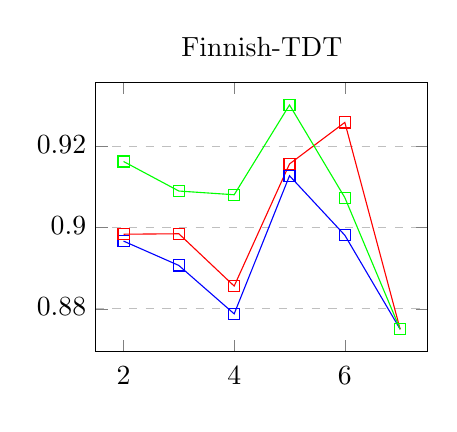
\begin{tikzpicture}
		\begin{axis}[
		name=finnish,
		title={Finnish-TDT},
		xlabel={},
		ylabel={},
		typeset ticklabels with strut,
		legend pos=south west,
		ymajorgrids=true,
		grid style=dashed,
		height=5cm
		]
		
		\addplot[
		color=blue,
		mark=square,
		]
		coordinates {(2, 0.8967012252591895)(3, 0.8906992532247114)(4, 0.8787878787878788)(5, 0.9127906976744186)(6, 0.8981481481481481)(7, 0.875)};
		
		\addplot[
		color=red,
		mark=square,
		]
		coordinates {(2, 0.8983977379830349)(3, 0.8985064494229463)(4, 0.8856304985337243)(5, 0.9156976744186046)(6, 0.9259259259259259)(7, 0.875)};
		
		\addplot[
		color=green,
		mark=square,
		]
		coordinates {(2, 0.9163053722902922)(3, 0.9090291921249152)(4, 0.9081133919843597)(5, 0.9302325581395349)(6, 0.9074074074074074)(7, 0.875)};
	
		\end{axis}
		\end{tikzpicture}
		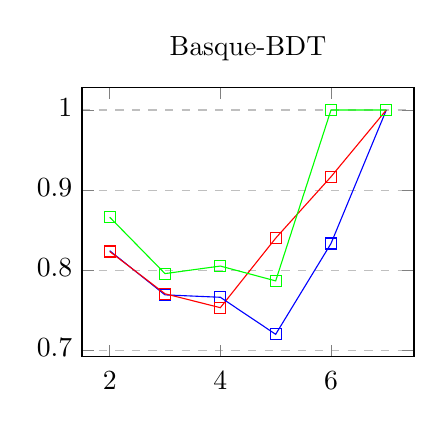
\begin{tikzpicture}
		\begin{axis}[
		name=basque,
		title={Basque-BDT},
		xlabel={},
		ylabel={},
		typeset ticklabels with strut,
		legend pos=south west,
		ymajorgrids=true,
		grid style=dashed,
				height=5cm
		]
		
		\addplot[
		color=blue,
		mark=square,
		]
		coordinates {(2, 0.8243201000312598)(3, 0.7692307692307693)(4, 0.7662337662337663)(5, 0.72)(6, 0.8333333333333334)(7, 1.0)};
		
		\addplot[
		color=red,
		mark=square,
		]
		coordinates {(2, 0.8233823069709284)(3, 0.7705922396187883)(4, 0.7532467532467533)(5, 0.84)(6, 0.9166666666666666)(7, 1.0)};
		
		\addplot[
		color=green,
		mark=square,
		]
		coordinates {(2, 0.8662081900593935)(3, 0.7957794417971409)(4, 0.8051948051948052)(5, 0.7866666666666666)(6, 1.0)(7, 1.0)};
		\end{axis}
		\end{tikzpicture}
		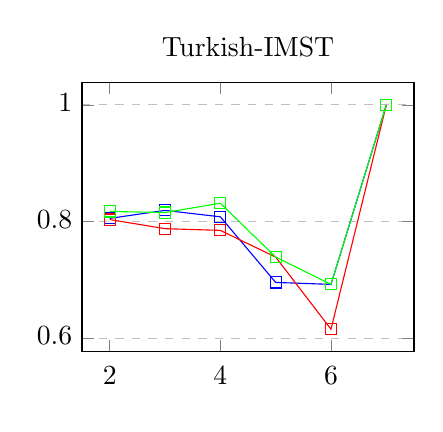
\begin{tikzpicture}
		\begin{axis}[
		name=turkish,
		title={Turkish-IMST},
		xlabel={},
		ylabel={},
		typeset ticklabels with strut,
		legend pos=south west,
		ymajorgrids=true,
		grid style=dashed,
		height=5cm
		]
		
		\addplot[
		color=blue,
		mark=square,
		]
		coordinates {(2, 0.8054268696227663)(3, 0.8191881918819188)(4, 0.8081395348837209)(5, 0.6956521739130435)(6, 0.6923076923076923)(7, 1.0)};
		
		\addplot[
		color=red,
		mark=square,
		]
		coordinates {(2, 0.8034414295168762)(3, 0.7878228782287823)(4, 0.7848837209302325)(5, 0.7391304347826086)(6, 0.6153846153846154)(7, 1.0)};
		
		\addplot[
		color=green,
		mark=square,
		]
		coordinates {(2, 0.8173395102581072)(3, 0.8154981549815498)(4, 0.8313953488372093)(5, 0.7391304347826086)(6, 0.6923076923076923)(7, 1.0)};
		\end{axis}
		\end{tikzpicture}
		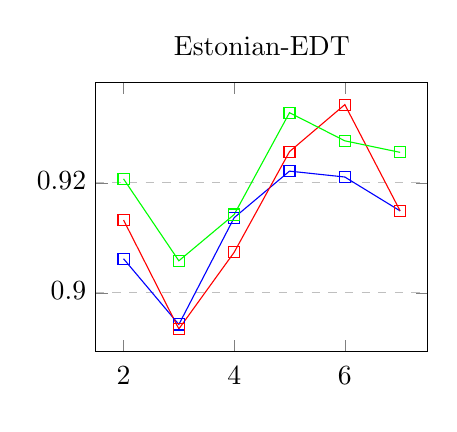
\begin{tikzpicture}
		\begin{axis}[
		name=estonian,
		title={Estonian-EDT},
		xlabel={},
		ylabel={},
		typeset ticklabels with strut,
		legend pos=south west,
		ymajorgrids=true,
		grid style=dashed,
		height=5cm
		]
		
		\addplot[
		color=blue,
		mark=square,
		]
		coordinates {(2, 0.9061969439728353)(3, 0.8942561396387254)(4, 0.9136649514008005)(5, 0.9221238938053097)(6, 0.9210526315789473)(7, 0.9148936170212766)};
		
		\addplot[
		color=red,
		mark=square,
		]
		coordinates {(2, 0.9132427843803056)(3, 0.8934442865841282)(4, 0.9073756432246999)(5, 0.9256637168141593)(6, 0.9342105263157895)(7, 0.9148936170212766)};
		
		\addplot[
		color=green,
		mark=square,
		]
		coordinates {(2, 0.9207130730050934)(3, 0.9058250456667343)(4, 0.9142367066895368)(5, 0.9327433628318584)(6, 0.9276315789473685)(7, 0.925531914893617)};
		\end{axis}
		\end{tikzpicture}
		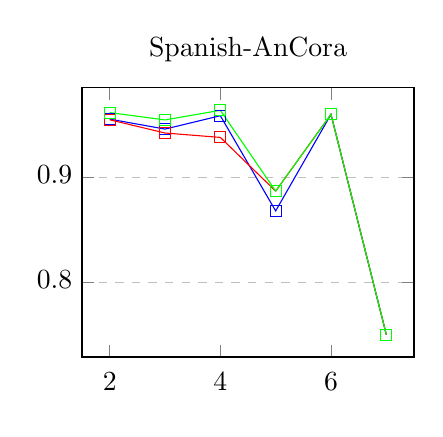
\begin{tikzpicture}
		\begin{axis}[
		name=spanish,
		title={Spanish-AnCora},
		xlabel={},
		ylabel={},
		typeset ticklabels with strut,
		legend pos=south west,
		ymajorgrids=true,
		grid style=dashed,
		height=5cm
		]
		
		\addplot[
		color=blue,
		mark=square,
		]
		coordinates {(2, 0.955400523234085)(3, 0.9459234608985025)(4, 0.958656330749354)(5, 0.8679245283018868)(6, 0.96)(7, 0.75)};
		
		\addplot[
		color=red,
		mark=square,
		]
		coordinates {(2, 0.9547776255138907)(3, 0.9421797004991681)(4, 0.937984496124031)(5, 0.8867924528301887)(6, 0.96)(7, 0.75)};
		
		\addplot[
		color=green,
		mark=square,
		]
		coordinates {(2, 0.9616295004360284)(3, 0.9546589018302829)(4, 0.9638242894056848)(5, 0.8867924528301887)(6, 0.96)(7, 0.75)};
		\end{axis}
		\end{tikzpicture}
		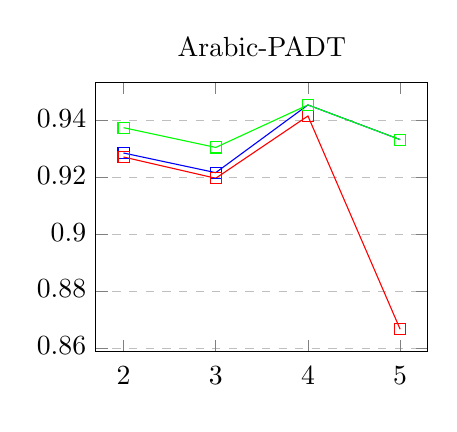
\begin{tikzpicture}
		\begin{axis}[
		name=arabic,
		title={Arabic-PADT},
		xlabel={},
		ylabel={},
		typeset ticklabels with strut,
		legend pos=south west,
		ymajorgrids=true,
		grid style=dashed,
		height=5cm,
		]
		
		\addplot[
		color=blue,
		mark=square,
		]
		coordinates {(2, 0.9286291953093408)(3, 0.9217134416543574)(4, 0.9455252918287937)(5, 0.9333333333333333)};
		
		\addplot[
		color=red,
		mark=square,
		]
		coordinates {(2, 0.9272139102304893)(3, 0.9197439684884293)(4, 0.9416342412451362)(5, 0.8666666666666667)};

		\addplot[
		color=green,
		mark=square,
		]
		coordinates {(2, 0.9375252729478366)(3, 0.930576070901034)(4, 0.9455252918287937)(5, 0.9333333333333333)};
		\end{axis}
		\end{tikzpicture}
		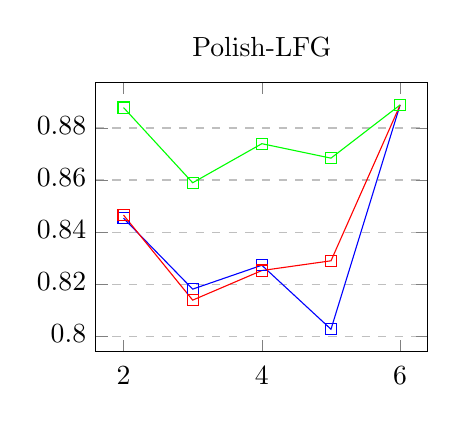
\begin{tikzpicture}
		\begin{axis}[
		name=polish,
		title={Polish-LFG},
		xlabel={},
		ylabel={},
		typeset ticklabels with strut,
		legend pos=south west,
		ymajorgrids=true,
		grid style=dashed,
		height=5cm
		]
		
		\addplot[
		color=blue,
		mark=square,
		]
		coordinates {(2, 0.8453280318091452)(3, 0.8180535966149506)(4, 0.8272357723577236)(5, 0.8026315789473685)(6, 0.8888888888888888)};
		
		\addplot[
		color=red,
		mark=square,
		]
		coordinates {(2, 0.8465208747514911)(3, 0.8138222849083215)(4, 0.8252032520325203)(5, 0.8289473684210527)(6, 0.8888888888888888)};
		
		\addplot[
		color=green,
		mark=square,
		]
		coordinates {(2, 0.8878727634194831)(3, 0.8589562764456982)(4, 0.8739837398373984)(5, 0.868421052631579)(6, 0.8888888888888888)};
		\end{axis}
		\end{tikzpicture}
		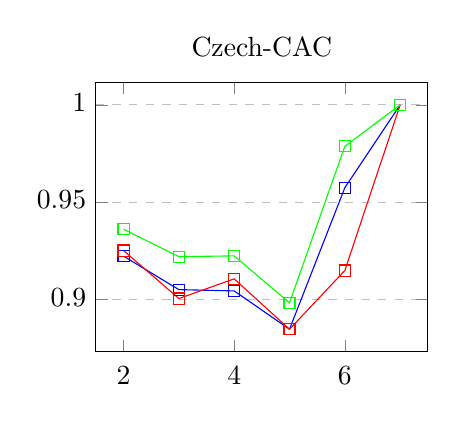
\begin{tikzpicture}
		\begin{axis}[
		name=czech,
		title={Czech-CAC},
		xlabel={},
		ylabel={},
		typeset ticklabels with strut,
		legend pos=south west,
		ymajorgrids=true,
		grid style=dashed,
		height=5cm,
		]
		
		\addplot[
		color=blue,
		mark=square,
		]
		coordinates {(2, 0.9222981315334595)(3, 0.9050979008643499)(4, 0.9044406970207982)(5, 0.8847457627118644)(6, 0.9574468085106383)(7, 1.0)};
		
		\addplot[
		color=red,
		mark=square,
		]
		coordinates {(2, 0.9251790270804181)(3, 0.9005115540659728)(4, 0.9106239460370995)(5, 0.8847457627118644)(6, 0.9148936170212766)(7, 1.0)};
		
		\addplot[
		color=green,
		mark=square,
		]
		coordinates {(2, 0.9361264301588608)(3, 0.9220321044275887)(4, 0.9224283305227656)(5, 0.8983050847457628)(6, 0.9787234042553191)(7, 1.0)};
		\end{axis}
		\end{tikzpicture}
		\caption{\label{fig:bpe_lens} Per language accuracy of tokens composed of more than two BPE tokens. The x-axis indicate how many BPE tokens a word is composed of and the y-axis the accuracy. The different methods are distinguished by color, where Blue is the summation method, red the mean and green RNN.}
	\end{figure}

	
	
	\section{Discussion}
        %We can observe an interesting trend for the treebank samples. For the languages with agglutinative morphology\footnote{1-to-1 correspondence between morphemes and grammatical/syntactic features.} the average increase using RNN compared to Mean is 4.3\%. For the fusional\footnote{1-to-many correspondence between morphemes and grammatical/syntactic features.} languages, the difference between RNN and Mean is only 1.1\%. 
        
        %Interestingly, this observation seem task-dependant rather than BPE dependant. We can see in \cref{tab:data} that Czech is a fusional language, but with a BPE-to-word ratio ($1.77$) comparable to the agglutinative languages. But, Czech also exhibit the pattern of benefiting less from RNN than from Mean, indicating that fusional languages\footnote{In our language/treebank sample.} regardless of BPE-to-word ratio is less affected by the composition method than agglutinative languages. 
        
        %In general, the agglutinative languages have a higher BPE-to-word ratio, with one exception, Czech. Czech have a BPE-to-word ratio of $1.77$, but still exhibit a lower difference between the RNN and mean method. Thus, from this small sample of treebanks it appears as if the method of combining BPE embeddings is more important for agglutinative languages than for fusional languages. 
        
        Analogously to character embeddings, the RNN method seem to provide stronger results than using either Sum or Mean for combining BPE tokens. We hypothesize that this is because Sum or Mean don't respect the ordering of elements within a word, that is, we don't relate the values of $BPE_0$ to $BPE_{1:N}$ with respect to the morphological tags. 
    
    \section{Conclusions}
        	As a general summary of our work, show that using an LSTM
     to combine BPE embeddings consistently, and across different
     languages, show better performance than summing or averaging the
     BPE embeddings.
	
	%\section*{Acknowledgments}
	
	
	% include your own bib file like this:
	\bibliographystyle{coling}
	\bibliography{coling2020}
	
\end{document}
